\documentclass[12pt,a4paper]{article}
\usepackage[utf8]{inputenc}
\usepackage[spanish]{babel}
\usepackage{graphicx}
\usepackage{listings}
\usepackage{xcolor}
\usepackage{hyperref}
\usepackage{float}
\usepackage[margin=2.5cm]{geometry}

% Configuración de colores para códigos
\definecolor{codegreen}{rgb}{0,0.6,0}
\definecolor{codegray}{rgb}{0.5,0.5,0.5}
\definecolor{codepurple}{rgb}{0.58,0,0.82}
\definecolor{backcolour}{rgb}{0.95,0.95,0.92}

\lstdefinestyle{mystyle}{
    backgroundcolor=\color{backcolour},   
    commentstyle=\color{codegreen},
    keywordstyle=\color{magenta},
    numberstyle=\tiny\color{codegray},
    stringstyle=\color{codepurple},
    basicstyle=\ttfamily\footnotesize,
    breakatwhitespace=false,         
    breaklines=true,                 
    captionpos=b,                    
    keepspaces=true,                 
    numbers=left,                    
    numbersep=5pt,                  
    showspaces=false,                
    showstringspaces=false,
    showtabs=false,                  
    tabsize=2
}

\lstset{style=mystyle}

\begin{document}
% Portada
\begin{titlepage}
    \centering
    \vspace*{1cm}
    
\includegraphics[width=0.8\linewidth]{espe.png}\\[0.5cm]
    
    \Large \textbf{Departamento de Ciencias de la Computación}\\
    \large \textbf{Universidad de las Fuerzas Armadas - ESPE}\\[0.5cm]
    
    \Huge \textbf{Práctica de Laboratorio No. 1}\\[0.3cm]
    \Large \textbf{Análisis de Amenazas y vulnerabilidades en un servidor Web}\\[0.8cm]
    
    \textbf{Nombres:}\\
    Yeshua Amador Chiliquinga Amaya\\
    Cesar Ignacio Loor Mercado\\[0.3cm]
    
    \textbf{Carrera / Asignatura:} Ingeniería de Software / Ingeniería de Seguridad de Software\\
    \textbf{NRC:} 23358\\
    \textbf{Nombre del profesor:} Walter Fuertes, PhD\\[0.5cm]
    
    \textbf{Fecha de presentación:} 24 de mayo del 2025\\[1cm]    
    \vfill
\end{titlepage}
% Índice de contenido

\tableofcontents
\newpage

\section{Objetivo}
El objetivo de esta actividad es introducir a los estudiantes en el proceso de identificación de amenazas, vulnerabilidades y riesgos en un entorno controlado, utilizando Kali Linux y un escenario de red virtualizado en VirtualBox.

\section{Requerimientos}
\begin{itemize}
    \item Kali Linux (instalado en una máquina virtual en VirtualBox).
    \item Equipo servidor vulnerable (puede ser una máquina vulnerable como Metasploitable2 o OWASP Broken Web Applications).
    \item Equipo cliente, puede ser Ubuntu Desktop 24.04.2 LTS.
    \item VirtualBox o cualquier otra herramienta de virtualización para gestionar las máquinas virtuales.
    \item Acceso a Internet para descarga de herramientas y recursos.
\end{itemize}

\section{Entorno Virtual de Red}
\begin{itemize}
    \item Máquina 1: Kali Linux (máquina atacante)
    \item Máquina 2: Ubuntu Server - Máquina vulnerable (Metasploitable2 o un servidor web vulnerable)
    \item Máquina 3: Ubuntu Desktop 24.04.2 LTS.
\end{itemize}

\section{Desarrollo}
\subsection{1. Reconocimiento de red}
En Kali Linux, vamos a realizar un escaneo de la máquina vulnerable para identificar los servicios abiertos, lo que nos ayudará a identificar posibles puntos débiles.

\subsubsection{1.1 Escaneo de puertos con Nmap}
En Kali Linux, abre una terminal y utiliza Nmap para realizar un escaneo de puertos:

\begin{lstlisting}[language=bash, caption=Escaneo básico con Nmap]
$ nmap -sV -T4 192.168.112.137
\end{lstlisting}

\begin{figure}[H]
    \centering
    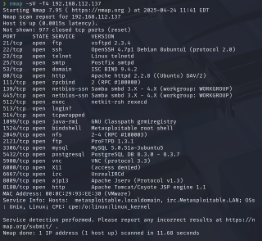
\includegraphics[width=0.9\textwidth]{nmap_scan.png}
    \caption{Resultado del escaneo Nmap}
    \label{fig:nmap_scan}
\end{figure}

\textbf{Explicación:}
\begin{itemize}
    \item \textbf{Amenaza:} Los servicios en la máquina vulnerable son posibles vectores de ataque.
    \item \textbf{Vulnerabilidad:} Algunos servicios, como HTTP o SSH, pueden estar desactualizados o mal configurados, lo que los hace vulnerables a ataques.
    \item \textbf{Riesgo:} Si un atacante logra explotar una vulnerabilidad en uno de esos servicios, podría comprometer la máquina vulnerable.
\end{itemize}

\textbf{Referencia Nmap:}
\begin{itemize}
    \item Nmap Documentation: \url{https://nmap.org/docs.html}
\end{itemize}

\subsection{2. Identificación de vulnerabilidades}
En esta etapa, utilizaremos Nmap (con sus scripts NSE) para buscar vulnerabilidades conocidas en los servicios detectados durante el escaneo previo.

\subsubsection{2.1 Uso de Nmap para detección de vulnerabilidades}
\textbf{Preparar entorno en Kali Linux}

Verifica que Nmap esté instalado (por defecto Kali lo incluye).
Actualiza la base de datos de scripts NSE para asegurarte de contar con las últimas comprobaciones:

\begin{lstlisting}[language=bash, caption=Actualización de scripts NSE]
$ sudo nmap --script-updatedb
\end{lstlisting}

\begin{figure}[H]
    \centering
    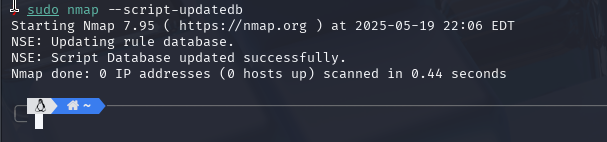
\includegraphics[width=0.9\textwidth]{nmap_script_update.png}
    \caption{Actualización de scripts NSE}
    \label{fig:nmap_script_update}
\end{figure}

\textbf{Escaneo de versiones y vulnerabilidades con el agrupador "vuln"}

\begin{lstlisting}[language=bash, caption=Escaneo de vulnerabilidades con NSE]
$ sudo nmap -sV --script=vuln -oN nmap_vuln_scan.txt 192.168.112.137
\end{lstlisting}

\begin{itemize}
    \item \texttt{-sV} - Detecta la versión de cada servicio en puertos abiertos.
    \item \texttt{--script=vuln} - Ejecuta todos los scripts NSE categorizados como "vuln".
    \item \texttt{-oN nmap\_vuln\_scan.txt} - Guarda el resultado en un archivo de texto.
\end{itemize}

\subsubsection{Escaneos dirigidos a vulnerabilidades específicas}
\textbf{Comprobación de SSL/TLS (Heartbleed, Poodle, etc.)}

\begin{lstlisting}[language=bash, caption=Escaneo de vulnerabilidades SSL/TLS]
$ sudo nmap -p 443 --script ssl-heartbleed,ssl-poodle -oN nmap_ssl_vulns.txt 192.168.112.137
\end{lstlisting}

\begin{figure}[H]
    \centering
    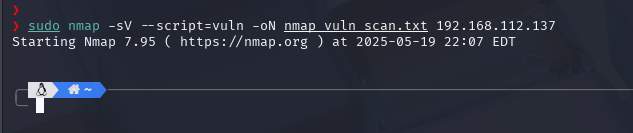
\includegraphics[width=0.9\textwidth]{ssl_scan.png}
    \caption{Resultado del escaneo de vulnerabilidades SSL/TLS}
    \label{fig:ssl_scan}
\end{figure}

\textbf{Verificación de SMB (MS08-067, MS17-010/EternalBlue, etc.)}

\begin{lstlisting}[language=bash, caption=Escaneo de vulnerabilidades SMB]
$ sudo nmap -p 139,445 --script smb-vuln-ms08-067,smb-vuln-ms17-010 -oN nmap_smb_vulns.txt 192.168.112.137
\end{lstlisting}

\begin{figure}[H]
    \centering
    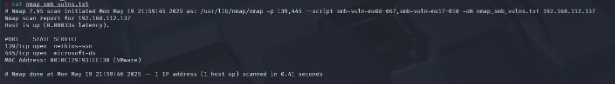
\includegraphics[width=0.9\textwidth]{smb_scan.png}
    \caption{Resultado del escaneo de vulnerabilidades SMB}
    \label{fig:smb_scan}
\end{figure}

\section{3. Explotación de una vulnerabilidad con Metasploit}
Una vez identificadas las vulnerabilidades, vamos a intentar explotarlas usando Metasploit, una herramienta de explotación automatizada.

\subsection{3.1 Uso de Metasploit para explotar una vulnerabilidad}
Por ejemplo, si descubrimos que un servicio HTTP es vulnerable a un Remote Code Execution (RCE), podemos usar Metasploit para explotarlo.

\begin{lstlisting}[language=bash, caption=Iniciando Metasploit]
$ msfconsole
\end{lstlisting}

\begin{figure}[H]
    \centering
    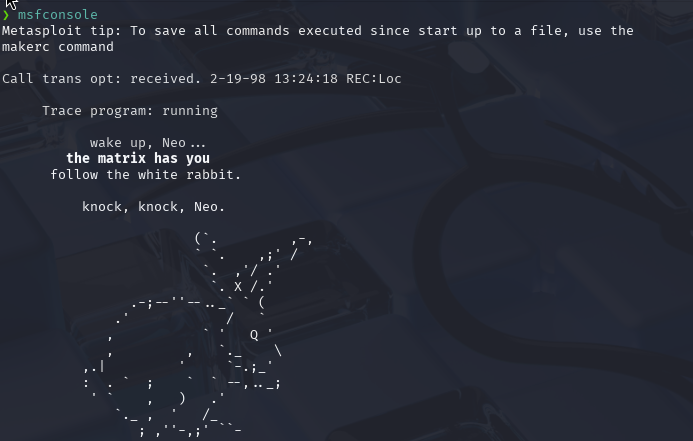
\includegraphics[width=0.9\textwidth]{metasploit_start.png}
    \caption{Consola de Metasploit}
    \label{fig:metasploit_start}
\end{figure}

Buscamos un exploit relacionado con el servicio identificado (por ejemplo, un servicio HTTP):

\begin{lstlisting}[language=bash, caption=Buscando exploits en Metasploit]
msf6 > search apache
\end{lstlisting}

\begin{figure}[H]
    \centering
    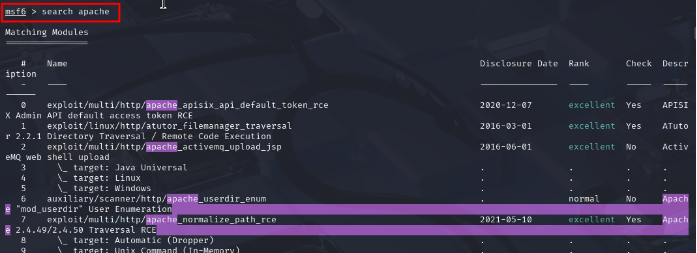
\includegraphics[width=0.9\textwidth]{metasploit_search.png}
    \caption{Resultado de búsqueda de exploits en Metasploit}
    \label{fig:metasploit_search}
\end{figure}

\textbf{Explicación:}
\begin{itemize}
    \item \textbf{Amenaza:} Si el atacante explota la vulnerabilidad, puede ejecutar comandos remotos en el servidor.
    \item \textbf{Vulnerabilidad:} El servidor web tiene una vulnerabilidad de ejecución remota de código debido a una mala configuración.
    \item \textbf{Riesgo:} El riesgo es que el atacante pueda tomar control total del servidor.
\end{itemize}

\textbf{Referencia Metasploit:}
\begin{itemize}
    \item Metasploit Documentation: \url{https://docs.metasploit.com/}
\end{itemize}

\section{Investigación}
En lugar de Metasploit, realiza la explotación de una vulnerabilidad con Nikto.

\begin{lstlisting}[language=bash, caption=Escaneo con Nikto]
$ nikto -h 192.168.112.137
\end{lstlisting}

\begin{figure}[H]
    \centering
    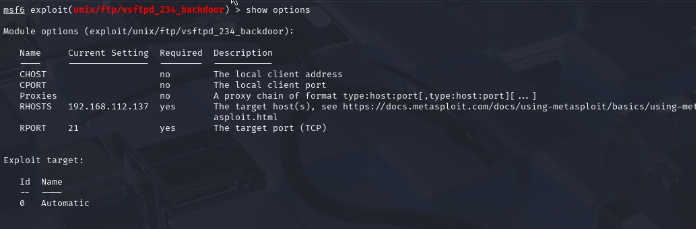
\includegraphics[width=0.9\textwidth]{nikto_scan.png}
    \caption{Resultado del escaneo con Nikto}
    \label{fig:nikto_scan}
\end{figure}

\textbf{Nikto documentation:} \url{https://www.kali.org/tools/nikto/}

\section{Discusión y conclusión}
\subsection{¿Qué amenazas se identificaron?}
Se identificaron varias amenazas potenciales, incluyendo la posibilidad de que un atacante ejecute código remoto en el servidor web, acceda a información sensible o realice ataques de denegación de servicio.

\subsection{¿Qué vulnerabilidades fueron explotadas?}
Entre las vulnerabilidades identificadas se encuentran servicios desactualizados, configuraciones inseguras en servicios web, y posibles vulnerabilidades en servicios como SMB y SSL/TLS.

\subsection{¿Cuál es el riesgo de no mitigar estas vulnerabilidades?}
Si no se corrigen estas vulnerabilidades, un atacante podría obtener acceso completo al sistema, robar información confidencial, instalar malware o utilizar el sistema comprometido como punto de partida para ataques a otros sistemas en la red.

\subsection{¿Cuál herramienta es mejor, NMAP, Metasploit, OpenVAS o Nikto?}
Cada herramienta tiene un propósito específico:
\begin{itemize}
    \item \textbf{NMAP:} Excelente para descubrimiento de hosts y servicios en una red.
    \item \textbf{Metasploit:} Potente para explotación de vulnerabilidades y pruebas de penetración.
    \item \textbf{OpenVAS:} Especializado en escaneo de vulnerabilidades con una base de datos extensa.
    \item \textbf{Nikto:} Específico para análisis de vulnerabilidades en servidores web.
\end{itemize}

\section{Resumen de la Actividad}
\begin{itemize}
    \item \textbf{Amenaza:} Es cualquier posible evento o situación que podría comprometer la seguridad de la red o los sistemas.
    \item \textbf{Vulnerabilidad:} Es una debilidad que puede ser explotada por una amenaza, como un servicio desactualizado o una mala configuración.
    \item \textbf{Riesgo:} Es la probabilidad de que una amenaza explote una vulnerabilidad, lo que puede resultar en daño al sistema o acceso no autorizado.
\end{itemize}

\section{Conclusiones}
Los participantes habrán aprendido cómo identificar, analizar y explotar vulnerabilidades en una red, comprendiendo la relación entre las amenazas, las vulnerabilidades y los riesgos. Utilizando herramientas como Nmap, Metasploit y Nikto en Kali Linux, habrán ganado experiencia práctica en pruebas de penetración y evaluación de seguridad en un entorno controlado.

\section*{Referencias Bibliográficas}
\begin{enumerate}
    \item OpenVAS: The Open Vulnerability Assessment System. (2012). Syngress Publishing. ISBN: 978-1-59749-574-5.
    \item Nikto: A Web Server Scanner. (2010). Packt Publishing. ISBN: 978-1-84951-019-3.
    \item The Penetration Tester's Guide. (2011). No Starch Press. ISBN: 978-1-59327-288-3
    \item Nmap Network Scanning: The Official Nmap Project Guide to Network Discovery and Security Scanning. (2009). Insecure Publishing. ISBN: 978-0-9799587-1-7.
    \item Nmap in the Enterprise: Your Guide to Network Scanning. (2008). Syngress Publishing. ISBN: 978-0-08-055874-5.
\end{enumerate}

\end{document}
